\documentclass[oneside, a4paper, onecolumn, 10pt]{article}

% Change this: Customize the title, author, advisor, abstract
\newcommand{\thesistitle}[0]{Linearization of Concurrent Data Structures}
\newcommand{\authorname}[0]{Mark Daychman}

\newcommand{\supervisor}[0]{Prof. Constantin Enea}
\newcommand{\supervisorinstitution}[0]{LIX \& CNRS}

\newcommand{\abstracttext}[0]{%
Lorem ipsum dolor sit amet, consectetur adipiscing elit, sed do eiusmod tempor incididunt ut labore et dolore magna aliqua. Ut enim ad minim veniam, quis nostrud exercitation ullamco laboris nisi ut aliquip ex ea commodo consequat. Duis aute irure dolor in reprehenderit in voluptate velit esse cillum dolore eu fugiat nulla pariatur. Excepteur sint occaecat cupidatat non proident, sunt in culpa qui officia deserunt mollit anim id est laborum.
}

\usepackage[
  left=2cm,top=2.0cm,bottom=2.0cm,right=2cm,
  headheight=17pt, % as per the warning by fancyhdr
  includehead,includefoot,
  heightrounded, % to avoid spurious underfull messages
]{geometry}

\usepackage{listings}
\usepackage{color}
\usepackage[dvipsnames]{xcolor}

\usepackage[T1]{fontenc}
\usepackage{algorithmicx}
\usepackage[noend]{algpseudocode}


\lstset{
  language=Python,
  % define words like max, min, for, except as black
  basicstyle=\color{black}\ttfamily\footnotesize,
  numberstyle=\color{gray},
  commentstyle=\color{OliveGreen}\bfseries,
  emph={[1]reversed}, emphstyle={[1]\color{black}},
  morekeywords={def,from,import,pass,return,try,continue, for,except,in,and, or,if,else, elif},
   keywordstyle=\color{purple} \bfseries,
  emph={[3]exec, values, items, copy, popFirst,extend, deepcopy, defaultdict, min, max, append, add, sort,intersects},emphstyle={[3]\color{BlueViolet} \bfseries},
  showstringspaces=false,
  emph={[4],int, bool, Call, List,Set, Dict, I, State, True, False, Call, CallWrite, CallRead, CallCAS}, emphstyle={[4]\color{Orange}\bfseries},
  breaklines=true,
  emph={[5]dfs, linearize_generic, CAS, sort_by_thread, make_intervals, io_check, intra_group_check, inter_group_check, topological_true_cas_sort}, emphstyle={[5]\color{blue} \bfseries},
  prebreak=\mbox{{\color{gray}\tiny$\searrow$}},
  numbers=left,
  xleftmargin=25pt
}


\lstnewenvironment{python}[1][]
{
\pythonstyle
\lstset{#1}
}
{}

\algblock[TryCatchFinally]{try}{endtry}
\algcblock[TryCatchFinally]{TryCatchFinally}{finally}{endtry}
\algcblockdefx[TryCatchFinally]{TryCatchFinally}{catch}{endtry}
	[1]{\textbf{catch} #1}
	{}

\algrenewcomment[1]{\(\triangleright\) #1}
\algnewcommand{\LineComment}[1]{\State // #1}
\algnewcommand{\Continue}{\State \textbf{continue}}
\algnewcommand\algorithmicswitch{\textbf{switch}}
\algnewcommand\algorithmiccase{\textbf{case}}

% New "environments"
\algdef{SE}[SWITCH]{Switch}{EndSwitch}[1]{\algorithmicswitch\ #1\ \algorithmicdo}{\algorithmicend\ \algorithmicswitch}%
\algdef{SE}[CASE]{Case}{EndCase}[1]{\algorithmiccase\ #1}{\algorithmicend\ \algorithmiccase}%
\algtext*{EndSwitch}%
\algtext*{EndCase}%
\usepackage{subfig}
\usepackage{amstext}
\usepackage{amsmath}
\usepackage{amssymb}
\usepackage{url}
\usepackage{graphicx}
\usepackage{wrapfig}
\usepackage{enumerate}
\usepackage{paralist}
\usepackage{xspace}
\usepackage{varwidth}
\usepackage{times}
\usepackage[colorlinks,linkcolor=blue]{hyperref}
\usepackage[colorinlistoftodos,prependcaption,textsize=normal]{todonotes}
\usepackage{pdfpages}
\usepackage{fancyhdr} %% For changing headers and footers
\usepackage{titling}
\usepackage[nottoc,numbib]{tocbibind}

%% \predate{}
%% \postdate{}
%% \date{}
%% \author{\authorname}


\begin{document}

%\title{\thesistitle}

%\maketitle

% Max 10 lines.
%\noindent \paragraph*{Abstract}
%\abstract

\hspace{0pt}
\vfill

\begin{center}

  
\includegraphics[width=0.3\textwidth]{logo-EP-vertical}

  \vspace*{2em}
  %
  {\large
    \textbf{\'Ecole Polytechnique}

    \vspace*{1em}
    \textit{BACHELOR THESIS IN COMPUTER SCIENCE}


    \vspace*{3em}
    {\Huge \textbf{\thesistitle}}
    \vspace*{3em}



    \textit{Author:}

    \vspace*{1em}
    \authorname{}, \'Ecole Polytechnique

    \vspace*{2em}
    %
    {\textit{Advisor:}}

    \vspace*{1em}
    \supervisor{}, \supervisorinstitution{}
  }

  \vspace*{2em}
  \textit{Academic year 2022/2023}

\end{center}

\vfill
\hspace{0pt}

\newpage

\vfill
\noindent\textbf{Abstract}\\[1em]
%
\fbox{
  \parbox{\textwidth}{
    \abstracttext{}
  }
}
\vfill


\newpage

% Setting up the header
\pagestyle{fancy}
%\renewcommand{\headrulewidth}{0pt} % Remove line at top
%\renewcommand{\headrulewidth}{0.4pt}% Default \headrulewidth is 0.4pt
\lhead{\authorname}
%\chead{\acronym}
\rhead{\thesistitle}



\newpage
\tableofcontents
\newpage

%\pagenumbering{arabic}

\section{Introduction}

\subsection{Introduction of Concurrency and Consistency Models}

Concurrency is an ability of a system to execute parts of the program in a different order without affecting the final result. These parts can be physically executed at the same time on different cores of a CPU (parallel computing) or they can execute on the same core by, for example, interleaving their execution (concurrent computing), but at all times on one computation takes place. The main goal of concurrent algorithms is to achieve the same result as the sequential algorithm, but in a shorter time. The problem that arise when two concurrently executing threads attempt to communicate and share some common resource. Potential problems include race conditions (when a thread reads a value that is then updated by another thread, rendering all further operations of the first thread invalid) or deadlocks (when two threads are waiting for each other to release a resource). On top of that the number of execution paths in a concurrent program grows exponentially, and the result can be indeterminant.\\\\
The problems that may arise during concurrent calculations motivate the creation of consistency models that specify how different threads can interact with these shared resources to ensure accurate results. One of the fundamental consistency models is sequential consistency. This model informally states that all operations within a single thread or core are executed in the order they appear in the program, but the order of the threads themselves is undefined. The main benefit of sequential consistency is that it provides a simple and intuitive model for understanding the behavior of concurrent programs. The programmer can reason about the program's execution as if it were a single sequential program, which makes it easier to develop and debug concurrent programs. Additionally, sequential consistency ensures that all threads observe the same order of operations, which can prevent errors such as race conditions and deadlocks. However, sequential consistency also has its drawbacks. It can result in significant performance overheads because of the need for synchronization and communication between threads, which can limit parallelism. This can make it difficult to scale concurrent programs to take advantage of multiple processor cores or distributed computing environments. Additionally, the strict ordering of operations required by sequential consistency can limit the flexibility of concurrent program execution, making it more challenging to optimize for performance. \\\\
A stronger consistency model is linearizability, defined by Herlihy and Wing. \cite{HerlihyWing} "Linearizability provides the illusion that each operation applied by concurrent processes takes effect instantaneously at some point between its invocation and its response, implying that the meaning of a concurrent object’s operations can be given by pre- and post-conditions." (Herlihy and Wing, 1987) Two of the greatest advantages of linearizability over a sequential model is that it is compositional and non-blocking. Compositionality means that if linearizability of operations is proved for several programs separately, then the programs together will also be linearizable. In a linearizable program the launched operations do not require other operations to be launched for their termination. This is the property of non-blockability.
\subsection{Non-blocking Algorithms and Atomic Operations}

There are some classic approaches to combatting the problems of concurrency. One of them is to use locks. Locks are a mechanism for controlling access to a shared resource. A lock can be in one of two states: locked or unlocked. When a thread wants to access a shared resource, it first acquires the lock for that resource and only then reads from or modifies the memory. This prevents other threads from accessing the resource until the lock is released. The main problem with locks is that they can cause a thread to block, waiting for the lock to be released. This can cause a thread to wait indefinitely if another thread holding the lock crashes or is otherwise unable to release it. This is known as a deadlock. Additionally, locks can cause significant performance overheads because of the need for synchronization between threads.
Ideally, we do want our concurrent algorithms to not block when one of the threads fails and never releases the lock. Algorithms that have this property are called non-blocking. With few exceptions, non-blocking algorithms use atomic read-modify-write primitives that the hardware must provide, the most notable of which is compare and swap (CAS).[???] Atomic operations are operations that are guaranteed to be executed atomically by the hardware. This means that the operation will either complete in its entirety or not at all. This property is useful when implementing concurrent algorithms, because without the inefficiency of locks, we can be certain to avoid race conditions. The pseudocode for an atomic CAS is shown in Figure \ref{Atomic CAS}. Two other most commonly used atomic operations are atomic writes and reads, and some architectures even include more complex operations, such as atomic test-and-set and fetch-and-add, as well as store conditionals.[???] In reality, the mutex locks themselves, as well as other synchronization mechanisms like semaphores are implemented using atomic operations.[???]\\
\begin{figure}[h]
  \centering
  \begin{minipage}{0.65\textwidth}
    \centering
    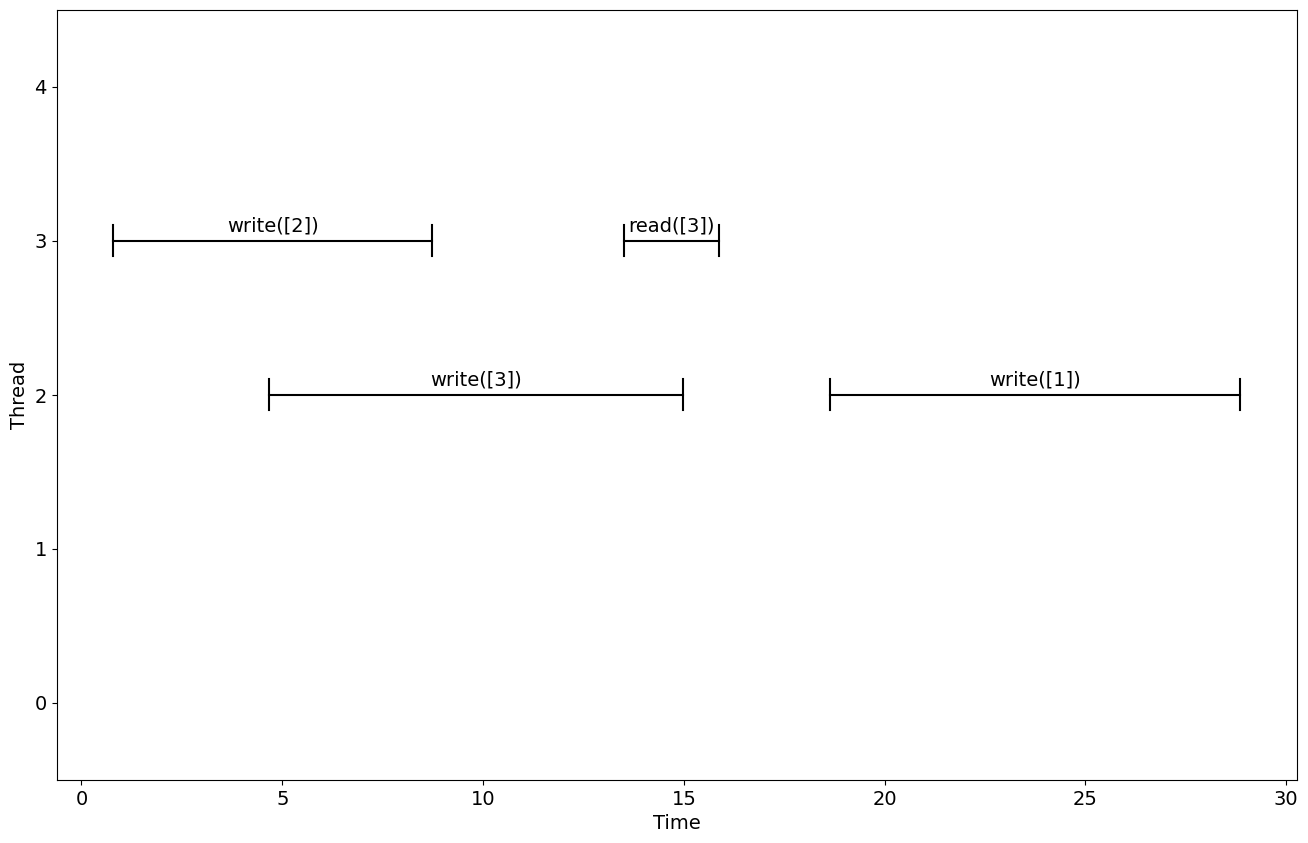
\includegraphics[width=0.9\textwidth]{assets/io_spec_simple.png}
    \caption{\label{Simple IO history}An example of a 2-thread history}
  \end{minipage}\hfill
  \begin{minipage}{0.3\textwidth}
    \centering
    \begin{algorithmic}
      \Function{CAS}{$ptr, old, new$}
      \If{$^*ptr\neq old}$
        \State \Return \textbf{False}
        \EndIf
        \State $^*ptr\gets new$
      \State \Return \textbf{True}
      \EndFunction
    \end{algorithmic}
    \caption{\label{Atomic CAS} Atomic CAS pseudocode}
  \end{minipage}
\end{figure}

\section{Checking Linearizability}
\subsection{Problem Introduction}
As stated before, linearizability of a sequential characterization, (also known as a history or a sequential specification), assumes that the effect of an operation takes place instantaneously at some moment between the call of the operation and its return. For simplicity, we can denote the call of that operation or function as an interval in time between its call and return. An example of a specification with 2 threads and 4 operations is given in Figure \ref{Simple IO history}.
In general, the problem of checking whether a specification is linearizable is NP-complete. [???]. However, for some sets of operations and under certain constraints this problem can be solved in polynomial time. A common example is a concurrent stack with queues and dequeues on unique values. In this paper, we will focus on linearizing the following set of operations under the given constraints:
\begin{itemize}
  \item \textbf{State.} The state represents a single shared resource, in our case a single memory cell storing an integer. The initial value of the state is undefined and must be set prior to any reads or compares.
  \item \textbf{Atomic read and write.} Writes set the value of the state to a new value, potentially overriding the value written previously. An important constraint is that writes are unique, meaning a value can only be written to memory once, and that value can never be written again. This constraint may seem excessive, but in reality, we can always apply versioning and use a unique identifier for each write without changing the output of the algorithm. On the other hand, this constraint allows us to reason about some partial order between the variables. There can be multiple reads on the same value, and reads do not in any way alter the state. To linearize a read, we just need to pick a point in time when the value of the state is equal to the value read.
  \item \textbf{True CAS.} Both true and false CASs have two arguments, the first being the value the CAS expects to be in memory and the second being the value to be written to memory if the compare succeeds. True CAS expects the compare to succeed. A true CAS is both a read and a write, but the two must come immediately one after another with no operation linearized in between.
  \item \textbf{False CAS.} A false CAS expects the compare to fail. In this case, the value of the state is not changed. A false CAS is in some sense the opposite of a read, as it can be linearized by all but one value. An additional constraint we put on false CASs is that there is always at least one read that has already returned on the compare value. This constraint arises from the practical uses [TODO]
\end{itemize}
To linearize a specification means to pick a unique linearization point within the interval of each operation, such that the resulting linearization is a valid execution of the program. For example, in Figure \ref{Simple IO history}, the linearization point of \verb|read(3)| must happen after that of \verb|write(3)|, as otherwise the read fails. Likewise, the intervals of \verb|write(2)| and \verb|write(3)| intersect, but since linearizing \verb|write(2)| after \verb|write(3)| would fail the read, we must linearize it before. Finally, the linearization point of \verb|write(1)| in all cases happens last. This forces a unique linearization: \verb|[write(2)|, \verb|write(3)|, \verb|read(3)|, \verb|write(1)]|. Notice how the location of linearization points forces a certain order of operations, so for simplicity, we will reason about the order of linearization rather than the exact location of the linearization points. Furthermore, the linearization order need not be unique.\\\\
\subsection{Brute Force Approach}
\begin{figure}
  \begin{algorithmic}[1]
    \Function{dfs}{$threads$, $state$}
    \State $res \gets \texttt{[]}$
    \State $first\_op\_per\_thread \gets$ list of first operations for each thread in $threads$
    \If{$first\_op\_per\_thread$ is empty}
    \State \Return $res$
    \EndIf
    \State
    \State $ref \gets$ operation with the earliest return in $first\_op\_per\_thread$
    \State $candidates \gets$ all operations in $first\_op\_per\_thread$ that intersect $ref$
    \For{$c$ in $candidates$}
    \State $new\_state, status \gets$ Execute $c$ on a copy of $state$
    \If{$status$ is \textbf{fail}} \hfill \Comment Unexpected value in memory, etc.
    \Continue
    \EndIf
    \State $threads.remove(c)$
    \State $sol \gets dfs(threads, new\_state$) \hfill
    \Comment Recursive step
    \State $threads.append(c)$
    \State $lin \gets [c] + sol$
    \State $res.append(lin)$

    \EndFor
    \State \Return $res$
    \EndFunction
    \State
    \Function{linearize\_generic}{$spec$, $state$}
    \State Sort $spec$ by thread and sort operations within each thread by the starting point
    \State \Return \Call{dfs}{sorted $spec$, $state$}
    \EndFunction

  \end{algorithmic}
  \caption{\label{Brute Force Algorithm} Brute force algorithm for linearizing a specification}
\end{figure}
\noindent



The obvious brute force approach to linearize a specification is to try all possible linearizations and check which ones are valid. This approach is obviously infeasible for large specifications, because of the exponential sample space, but it can be used to check small specifications. Programmatically, we sort the operations by thread number and within each thread by the starting point of each operation. We keep track some internal state depending on which kind of operations we are trying to linearize. We begin from the operation that starts the earliest, execute it and then first traverse all operations that intersect the current operation, otherwise if they were all explored, we move on to the next unexplored operation that starts the earliest. If during linearization, the execution throws an error, we backtrack. The pseudocode for the algorithm is given in Figure \ref{Brute Force Algorithm}.

\subsection{Atomic Read and Write}
\subsubsection{Introduction of Blocks and Intervals}
Atomic read and write are the simplest operations to linearize. First observation, we can make is that if we group all writes and reads on the same variable together into a dictionary \verb|sort_by_var| (key: variable, value: list of operations), then the write will always be linearized first and the reads will always be linearized directly after a corresponding write in any way that does not break the real-time order. In other words, to determine the linearization of the entire history, we only need to order the variables, as the order of operations on a variable is pre-determined. To reason about the order of variables, we can introduce \textbf{variable blocks}, a concept that will be used throughout this paper. Variable blocks are a list of lists of variables that defines some partial order on them. We traverse the blocks from left to right, and within each block, we can traverse the operations in any order. For example, the blocks \verb|[[1, 2], [3, 4]]| mean we would first linearize $1$ and $2$ together in any order, and only then linearize $3$ and $4$ again any order. Blocks are an efficient way to store everything we know about the linearization order at any given moment, and as we add new types of operations, the blocks can be gradually refined. The exact algorithm to build the blocks will be explained later, when the exact linearization order becomes more important. With only writes and reads, it is enough to only determine whether the history is linearizable at all. \\\\
To make the blocks we need to understand what forces a certain order of variables. First, we have the real time order, i.e. if there are two operations on two different variables, and the first operation returns before the second operation starts, then the first variable must go earlier. Second, if a write returns, but the read on the same variable happens later, during the interval between the return and the call, we are certain which value is written in the memory. To further reason about this, we can introduce \textbf{variable intervals}. A variable interval starts at the earliest return of an operation on that variable and ends on the latest call.
\begin{figure}[h]
  \centering
  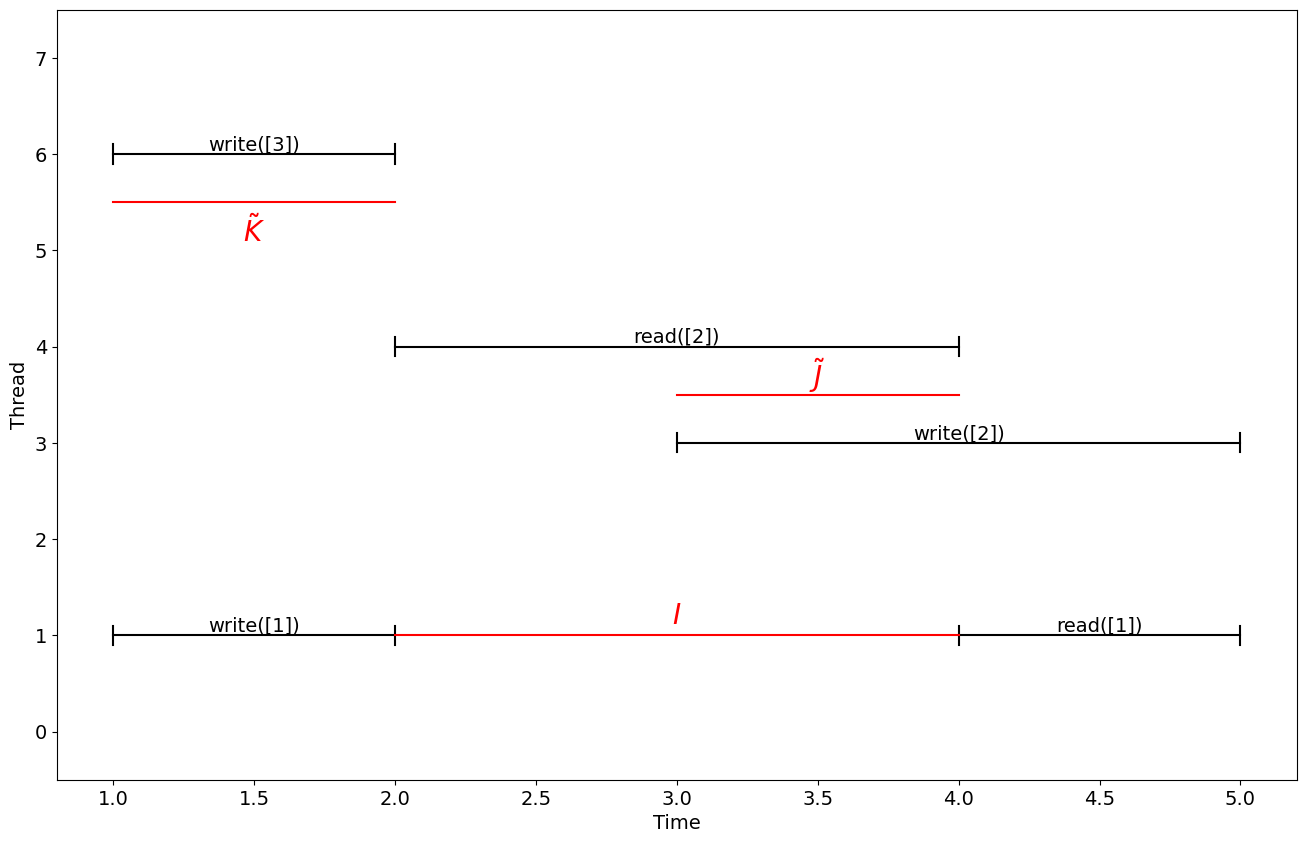
\includegraphics[width=0.9\textwidth]{assets/intervals_example.png}
  \caption{\label{Interval Examples}Examples of forward and reverse intervals}
\end{figure}
The intervals can be broadly divided into two types: forward and reverse, based on whether the latest call happens after or before the earliest return. One can see the forward interval $I$ and the reverse intervals $\tilde{J}$ and $\tilde{K}$ in Figure \ref{Interval Examples}. We will always denote a reverse interval by a tilde on the top. Notice that the read can start before a read starts, as long as they intersect, or there can be no read at all, but the intervals are still well-defined. Each interval type has its own interpretation. The forward intervals force the variable to be in memory during the interval. It does not mean that the value is only written to memory during it, it only means that during the interval, we are sure to have it written. The interpretation of reverse intervals is more loose, and we will assume that all linearization points on the given variable happen during the reverse interval. In reality, this does not need to be true, because we can occasionally linearize operations outside the interval, but this is never required and furthermore, we always want the linearization of a variable to be as short as possible, keeping the linearization points close to each other. So in practice, there is never a need to linearize operations outside the interval.
\begin{figure}[h]
  \begin{algorithmic}[1]
    \Function{make\_intervals}{$sort\_by\_var$}
    \State $intervals \gets \texttt{\{\}}$
    \For{$var, ops\_on\_var$ \textbf{in} $sort\_by\_var$}
    \State $i1 \gets \min(c.end \mid c \in ops\_on\_var)$
    \State $i2 \gets \max(c.start \mid c \in ops\_on\_var)$
    \If{$i1 < i2$}
    \State $intervals[var] \gets I(i1, i2)$
    \Else
    \State $intervals[var] \gets I(i2, i1, \text{reversed}=\textbf{True})$
    \EndIf
    \EndFor
    \State \Return $intervals$
    \EndFunction
  \end{algorithmic}
  \caption{\label{Interval-making}Interval construction algorithm}
\end{figure}
\subsubsection{Interval Check}
We are now ready to build the blocks. We first run basic checks on the history, i.e. checking that no read returns before a corresponding write starts and that there is exactly one variable per variable. Then we build the corresponding reverse and forward intervals for each variable. We consider every pair of a forward interval with another potentially reverse interval. We then have the following two cases:
\begin{itemize}
  \item \textbf{Forward + Forward Intervals} - the intervals cannot intersect at all. Since each forward interval forces the variable to be in memory, any intersection would mean that two different variables are written to the same memory at the same time.
  \item \textbf{Forward + Reverse Intervals} - the reverse interval cannot be contained in the forward interval. There is always at least one linearization point in the reverse interval, but if the forward interval contains it, then we are certain that a different variable is written to memory, so only operations on that variable can be linearized.
\end{itemize}
These two cases can be combined into one check:
\begin{figure}[h]
  \begin{center}
    \begin{algorithmic}[1]
      \Function{interval\_check}{$intervals$}
      \For{$forward\_interval$ \textbf{in} forward intervals of $intervals$}
      \For{$interval$ \textbf{in} $intervals$}
      \State $last\_call \gets$ time of the last call on the variable of $interval$
      \State $first\_return \gets$ time of the first return on the variable of $interval$
      \If{$first\_return < forward\_interval.end$ \textbf{and} \newline
        \hspace*{5.6em}$last\_call > forward\_interval.start$}
      \State \Return \textbf{False}
      \EndIf
      \EndFor
      \EndFor
      \State \Return \textbf{True}
      \EndFunction
    \end{algorithmic}
  \end{center}
  \caption{\label{IO linearization verifier}Writes/reads linearization verifier}
\end{figure}
\subsection{True CAS}
\subsubsection{Basic Checks and Sorting}
True CAS is a little more complicated, because we cannot simply replace it by a write and a read, since we need to additionally make sure that these operations execute strictly one after another. We will incorporate true CASes in the model of blocks and intervals to be able to reason about their impact on the order. First, let us consider some trivial cases involving true CAS that prevent the history from being linearizable all together. We cannot have a linearization if we have more than one CAS with the same compare argument, i.e. we cannot have \verb|1->2| and \verb|1->3|, because once either of these CASes is linearized, the value of 1 is lost and cannot be used again. We also cannot have loops of any length, e.g. \verb|1->2|, \verb|2->3|, \verb|3->1| is not allowed. Having loops would make it difficult to reason about any kind of order, and since any loop makes the history non-linearizable, we can exclude this case directly. To find a loop we could consider each true CAS as two connected nodes of two values, and use any of the well-known cycle detection algorithms. \\\\
After these two checks, reasoning about ordering becomes easier, but we need to first understand in which order true CASes will be linearized among themselves. For this we can once again rely on the graph abstraction and use a topological search shown in figure \ref{Topological True CAS Sort}.
\begin{figure}[h]
  \begin{algorithmic}
    \Function{topological\_true\_cas\_sort}{$true\_cases$}
    \State $graph \gets \{c.compare: c.swap \mid c \in true\_cases\}$
    \State $var\_order \gets \texttt{[]}$
    \State $visited \gets \texttt{\{\}}$
    \Function{dfs}{$node$}
    \If{$node$ \textbf{in} $visited$}
    \State \Return
    \EndIf
    \State $visited.add(node)$
    \If{$node$ \textbf{in} $graph$}
    \State $dfs(graph[node])$
    \EndIf
    \State $var\_order.add(node)$
    \EndFunction
    \For{$node$ \textbf{in} $graph$}
    \State $dfs(node)$
    \EndFor
    \State Sort $true\_cases$ in-place in the reversed order of appearance in $var\_order$
    \EndFunction
  \end{algorithmic}
  \caption{\label{Topological True CAS Sort}Topological True CAS sort}
\end{figure}
\subsubsection{Block intergration}
\noindent
With true CASes sorted, we can observe that they form "chains" forcing a certain order between the variables. Unfortunately, we cannot just take these chains and convert them into blocks. Consider the history given in figure \ref{Problematic Blockization}. Two possible linearizations are \verb|write(1), 1->3, write(2), 2->4| and \verb|write(2), 2->4, write(1), 1->3|. However, defining the block is problematic, because $3$ must follow directly after $1$, but the group $(1,3)$ as a whole can be linearized before or after the group $(2,4)$. This is why when including true CASes in block, they are always given in a tuple specifying the whole chain. Therefore, the history in figure \ref{Problematic Blockization} corresponds to the blocks \verb|[[(1,3), (2,4)]]|.
\begin{figure}[h]
  \centering
  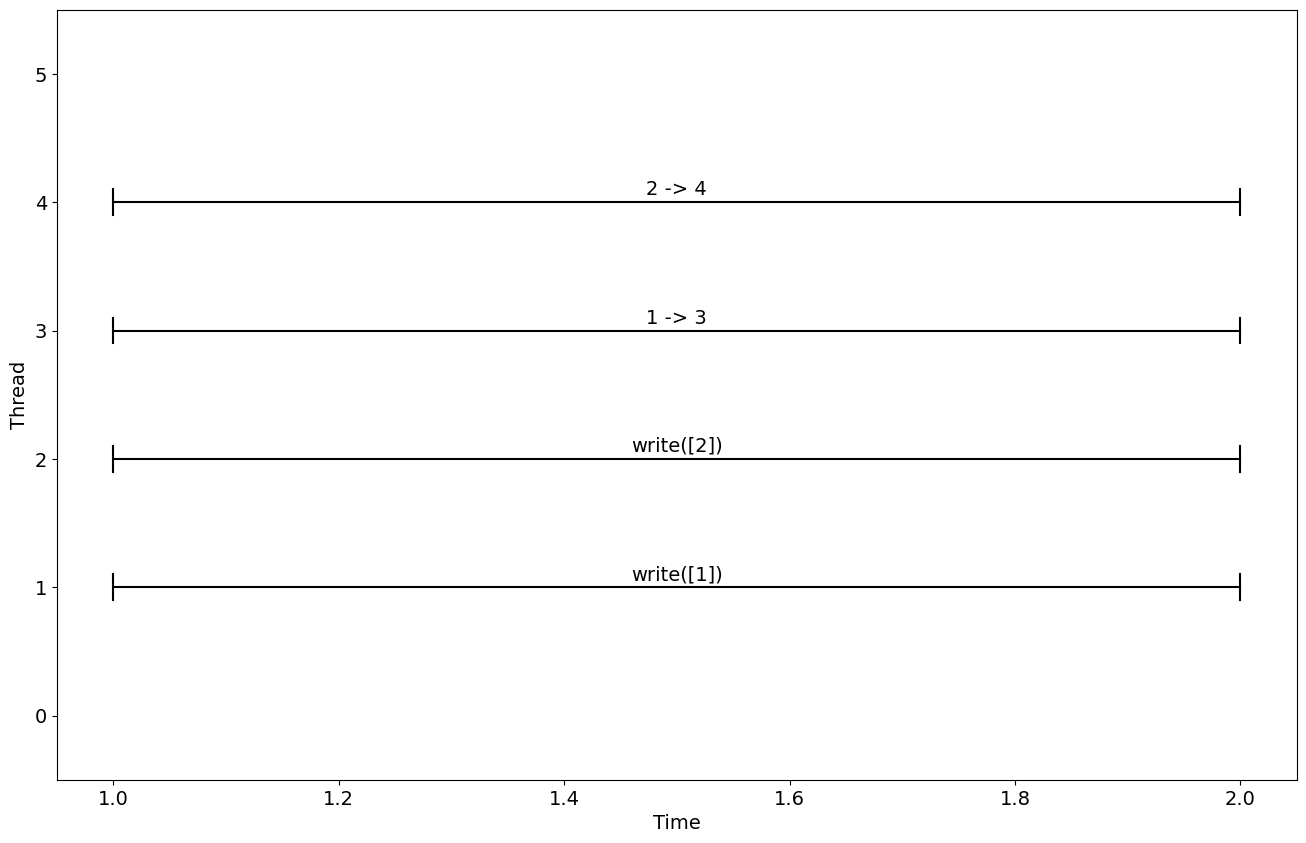
\includegraphics[width=0.8\textwidth]{assets/ambiguous_true_cas_order.png}
  \caption{\label{Problematic Blockization}Ambiguity in how we define blocks}
\end{figure}
\subsubsection{Intra- and inter- group checks}
Since true CASes impose an order of a certain chain of variables, to check whether the entire history is linearizable, we can first check if the the group alone is linearizable (intragroup check) and then if we consider the entire chain to be a single variable, whether it can fit with other operations by the means of the same interval check as in the previous part (intergroup check). The pseudocode for these checks is shown in figure \ref{IntraInter Group Checks}. Notice that unlike in the inter-check, we cannot simply run the interval check on the intragroup intervals, because it checks that the intervals can be linearized in any order, but we need to check that they can be linearized in the order given by the true CASes.

\begin{figure}[h!]
  \begin{algorithmic}[1]
    \Function{is\_valid\_order}{$intervals$, $order$}
    \For{$(i1, i2)$ \textbf{in} consecutive pairs of $order$}
    \State $earliest\_lin\_i1 \gets \textbf{ if } intervals.reversed  \textbf{ then } intervals[i1].start \textbf{ else } intervals[i1].end$
    \State $latest\_lin\_i2 \gets \textbf{ if } intervals.reversed  \textbf{ then } intervals[i2].end \textbf{ else } intervals[i2].start$
    \If{$earliest\_lin\_i1 > latest\_lin\_i2$}
    \State \Return \textbf{False}
    \EndIf
    \EndFor
    \State \Return \textbf{True}
    \EndFunction
    \State
    \Function{intra\_group\_check}{$sort\_by\_var, true\_cas\_var\_groups$}
    \For{$group$ \textbf{in} $true\_cas\_var\_groups$}
    \State $ops\_in\_group \gets \{sort\_by\_var[var] \mid var \in group\}$
    \State $intra\_group\_intervals \gets make\_intervals(ops\_in\_group)$
    \If{$is\_valid\_order(intra\_group\_intervals, order)$ is not \textbf{True}}
    \State \Return \textbf{False}
    \EndIf
    \EndFor
    \State \Return \textbf{True}
    \EndFunction
    \State
    \Function{inter\_group\_check}{$sort\_by\_var, true\_cas\_var\_groups$}
    \State $sort\_by\_var \gets$ deep copy of $sort\_by\_var$
    \For{$var\_group \gets true\_cas\_var\_groups$}
    \State $var \gets$ first element of $ var\_group$
    \For{$other\_var \gets $ other elements of $var\_group$}
    \State $sort\_by\_var[var].extend(sort\_by\_var[other\_var])$
    \State $sort\_by\_var.delete(other\_var)$
    \EndFor
    \EndFor
    \State $intervals \gets make\_intervals(sort\_by\_var)$
    \State \Return $interval\_check(intervals)$
    \EndFunction
  \end{algorithmic}
  \caption{\label{IntraInter Group Checks}Intra- and inter-group checks}
\end{figure}
\noindent
Instead, we can use a more efficient linear check that traverses each consecutive pair of true CASes, i.e. 1st and 2nd, 2nd and 3rd, etc. and checks whether the earliest time when we can fully linearize the first variable is before the latest time when we can linearize the second variable.
\subsection{False CAS}
\subsubsection{Block definition}
The false CAS is the hardest operation to linearize. It can be linearized with all but one value, so the impact on the linearization order is not as strong as with the true CAS. Unlike the true CASes that we treated almost independently of each other, a false CAS can have a slight change the order of variables at the beginning of the program, which will only have affects later on. It also breaks the logic of intervals, because we do not know ahead of time, which variable will linearize it with, and so we cannot build the proper intervals. Somehow we need to find all available variables that can linearize a false CAS, then add the false CAS to the corresponding variable group, build the intervals and run our usual checks. \\\\
The variables that can linearize a false CAS are called \textbf{resolvers}. However, to get a list of resolvers for each false CAS, we need to first understand how each false CAS affects the order of execution and encode this information in the blocks. Each block represents variables that can be linearized in any order. First observation we can make is that two variables with a forward interval can never be placed in the same block, because two forward intervals cannot intersect, so the one that starts first must also be linearized first.\\\\
Secondly, a reverse and a forward interval can put in the same block if and only if, the reverse interval fully contains the forward interval. Otherwise, if the reverse interval does not contain the start of the forward, the forward must be linearized first and vice versa if the reverse interval does not contain the end of the forward, the reverse must be linearized first. This property is also transitive - if there is a forward interval and two reverse intervals that contain it, then not only can the order of linearization between the forward and reverse intervals be switched, but all three operations can be linearized in any order. Consider the example in figure \ref{Forward Blocks Example}. Interval 2 fully contains interval 1, so they get placed in the same block. The interval 2 does not need to contain all the operations - \texttt{read(1)} ends outside of interval 1, but the interval 2 ends at the call of the read, so the condition is satisfied. On the other hand, interval 4 does not contain the interval 3 fully, so they get placed in different blocks.
\begin{figure}[h]
  \centering
  \begin{minipage}{0.5\textwidth}
    \centering
    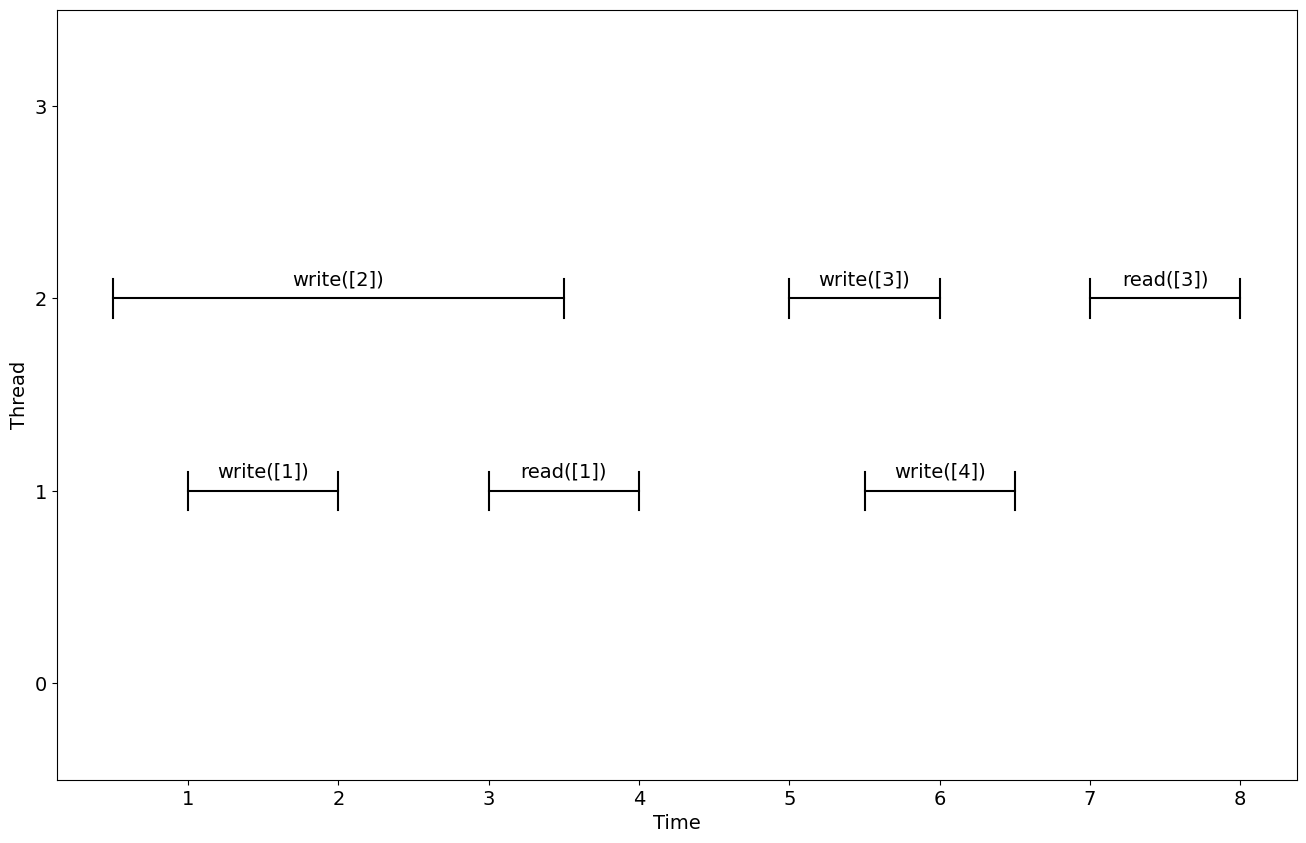
\includegraphics[width=\textwidth]{assets/forward_blocks.png}
    \caption{\label{Forward Blocks Example}Blocks \texttt{[[1,2], [4], [3]]}}
  \end{minipage}\hfill
  \begin{minipage}{0.5\textwidth}
    \centering
    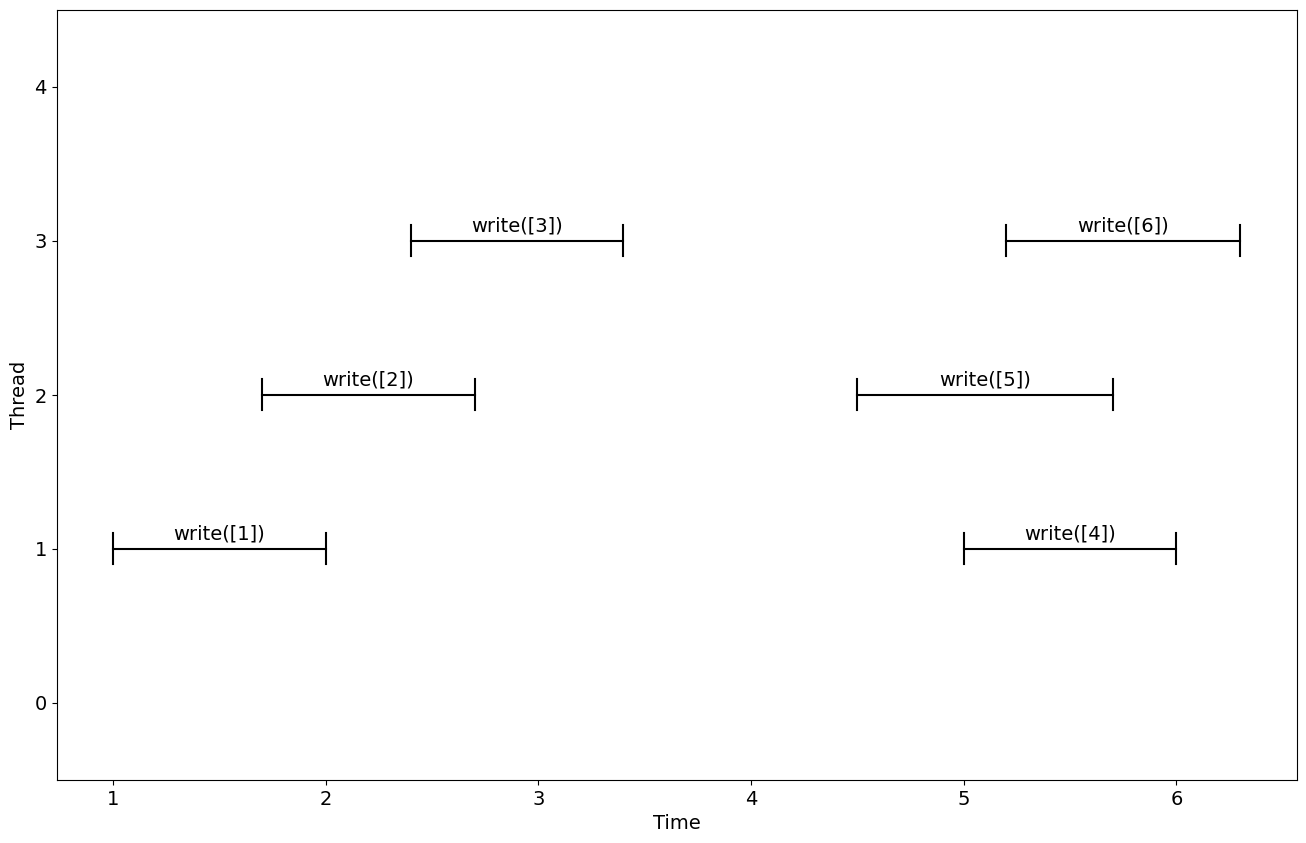
\includegraphics[width=\textwidth]{assets/reversed_blocks.png}
    \caption{\label{Reverse Blocks Example}Blocks \texttt{[[1,2], [2,3], [4,5,6]]}}
  \end{minipage}
\end{figure}
\begin{figure}[h]
  \begin{algorithmic}
    \Function{forward\_blocks}{$intervals$}
    \State $blocks \gets \texttt{[]}$
    \For{$forward\_var, forward\_interval \gets$ forward intervals of $intervals$}
    \State $block \gets [forward\_var]$
    \For{$reverse\_var, reverse\_interval \gets$ reverse intervals of $intervals$}
    \If{$forward\_interval \subseteq reverse\_interval$}
    \State $block.append(reverse\_var)$
    \State Mark $reverse\_var$ \hfill \Comment{This means this variable cannot form a block on its own. See below.}
    \EndIf
    \EndFor
    \State $blocks.append(block)$
    \EndFor
    \State \Return $blocks$
    \EndFunction
  \end{algorithmic}
  \label{Forward Blocks Algorithm}
  \caption{Forward blocks algorithm}
\end{figure}

\noindent
Finally, two reverse intervals can be placed in the same block if and only if they intersect. On top of that, their intersection cannot itself be contained inside another forward interval, because as we know no linearization points are possible inside a forward interval. Unfortunately, this property is not transitive (see figure \ref{Reverse Blocks Example}). Interval 1 intersects with interval 2, and 2 intersects with 3, but 1 does not intersect with 3. This means that the order of linearization between 1 and 3 cannot be switched. On the other hand, intervals 4, 5, 6 all intersect among themselves, so they can be placed in the same block. Finding maximal groups of reverse intervals is similar to finding maximal cliques in a graph. Unfortunately, the problem is NP-complete[???], so we cannot use this approach.
Instead, we pick an initial reverse interval with the earliest return time and pair it with all other reversed intervals in the order of their returns. We keep track of which of them our initial interval intersect. As before, the intersection cannot occur inside a forward interval. After we are done checking for intersections, we can make a block from the initial interval and all the intervals that intersect with it. We mark all the intervals in a block and delete the initial interval from the list of intervals as a whole. This is because we already found all the blocks the initial interval can potentially belong to, and there is no need to check it again. We repeat this process for a new initial interval, which ends after the previous one. Finally, we can never add a block if it is only made of marked intervals. Intervals get marked when they are added to the block in this step or in the previous step when they are joined with forward intervals. Furthermore, a reverse interval can be part of both forward and reverse blocks. The pseudocode for making reverse blocks is given in figure \ref{Reverse Blocks Algorithm}.
\begin{figure}[h]
  \begin{algorithmic}
    \Function{reverse\_blocks}{$intervals$}
    \State $blocks \gets \texttt{[]}$
    \State $reverse\_intervals \gets$ Sort reverse intervals by return time
    \For {$rev\_var1, rev\_i1$ \textbf{in }$ reverse\_intervals$}
    \State $block \gets [rev\_var1]$
    \For {$rev\_var2, rev\_i2$ \textbf{in }$ reverse\_intervals$}
    \State $intersection \gets rev\_i1 \cap rev\_i2$
    \If {$intersection \neq \emptyset$ \textbf{and} $intersection \not\subseteq$ any forward interval}
    \State $block.append(reverse\_var)$
    \EndIf
    \EndFor
    \If {$block \not\subseteq$ marked intervals}
    \State $blocks.append(block)$
    \State Mark all intervals in $block$
    \EndIf
    \EndFor
    \State \Return $blocks$
    \EndFunction
  \end{algorithmic}
  \label{Reverse Blocks Algorithm}
  \caption{Reverse blocks algorithm}
\end{figure}

\noindent
Before we make forward and reverse intervals, we need to incorporate true CAS chains shown in figure \ref{Problematic Blockization}. We do it similarly to intergroup checks - by merging all variables in a true CAS chain into a single interval. After that we can just treat the chain as a single variable. After the blocks are made, we can sort them in order of the earliest end point of any intervals in the block.
\begin{figure}[h]
  \begin{algorithmic}
    \Function{make\_blocks}{$intervals, true\_cas\_var\_groups$}
    \State $blocks \gets \texttt{[]}$
    \State \Comment{Step 1. Merge true CAS groups}
    \State $merged\_intervals \gets merge\_true\_cas\_groups(intervals, true\_cas\_var\_groups)$
    \State
    \State \Comment{Step 2.1 Skeleton. All forward intervals are placed in different blocks}
    \State \Comment{Step 2.2 Reversed intervals that contain a forward interval get added to the block and get marked.}
    \State $blocks.extend(forward\_blocks(merged\_intervals))$
    \State
    \State \Comment{Step 3. "Clique problem" - find maximal groups of reverse intervals that intersect}
    \State $blocks.extend(reverse\_blocks(merged\_intervals))$
    \State
    \State Sort $blocks$ by return time of the earliest interval in the block
    \State \Return $blocks$

    \EndFunction
  \end{algorithmic}
  \caption{Block-making algorithm}
\end{figure}
\subsubsection{False CAS Resolvers}
Blocks encode all the branching points in the program. We now have to further refine them further with false CASes. We first treat each false CAS independently and gather all writes that can resolve it. For that we traverse each block one by one. For each block we record  When any operation on any of the variables from the current block returns, we know that only the 

\newpage
\begin{figure}[h]
  \begin{algorithmic}
    \Function{block\_traversal}{$blocks$}

    \State INSERT THE PART ABOUT TRUE CASES

    \State $resolvers \gets \texttt{\{\}}$
    \For {$false\_cas$ \textbf{in }$ false\_cas\_vars$}
    \State $available\_writes \gets \texttt{[]}$
    \For {$block$ \textbf{in }$ blocks$}
    \State $candidates \gets$ All writes in the current block that start before false CAS returns
    \If{any operation in the current block returns before false CAS starts}
    \State $available\_writes \gets \texttt{[]}$
    \EndIf
    \State $available\_writes.extend(candidates)$
    \State $earliest\_forward\_lin\_t \gets$ latest end of a forward interval in the current block
    \State $earliest\_reverse\_lin\_t \gets$ latest start of a reverse interval in the current block
    \State 
    \State \Comment This is the earliest we can linearize the entire block
    \State $earliest\_block\_lin\_t \gets \max(earliest\_forward\_lin\_t, earliest\_reverse\_lin\_t)$
    \If{$false\_cas$ ends before $earliest\_block\_lin\_t$}
    \State \textbf{break}
    \EndIf
    \EndFor
    \State
    \State $available\_writes.discard(false\_cas.compare)$ 
    \State $resolvers[false\_cas] \gets available\_writes$
    \EndFor
    \State \Return $resolvers$
    \EndFunction
  \end{algorithmic}
  \caption{Block-making algorithm}
\end{figure}

\begin{figure}[h]
  \begin{algorithmic}
    \Function{propagate\_false\_cases}{$blocks, resolvers$}
    \State $blocked \gets$ All false CASes that start after their corresponding write ends
    \For {$false\_cas$ \textbf{in }$ false\_cases$}
    \For {$var$ \textbf{in }$ resolvers[false\_cas]$}
    \If {$var$ \textbf{in }$ blocked$ \textbf{and} $false\_cas$ starts after the false cas blocking $var$ ends}
    \State $resolvers[false\_cas].discard(var)$
    \EndIf
    \EndFor
    \EndFor
    \EndFunction
  \end{algorithmic}
  \caption{Block-making algorithm}
\end{figure}

\begin{figure}[h]
  \begin{algorithmic}
    \Function{propagate\_false\_cases}{$blocks, resolvers$}
    \State $blocked \gets$ All false CASes that start after their corresponding write ends
    \For {$false\_cas$ \textbf{in }$ false\_cases$}
    \For {$var$ \textbf{in }$ resolvers[false\_cas]$}
    \If {$var$ \textbf{in }$ blocked$ \textbf{and} $false\_cas$ starts after the false cas blocking $var$ ends}
    \State $resolvers[false\_cas].discard(var)$
    \EndIf
    \EndFor
    \EndFor
    \EndFunction
  \end{algorithmic}
  \caption{Block-making algorithm}
\end{figure}
\subsubsection{Additional Constraint}
\subsection{Ordering}
\section{Testing}
Tests are generated automatically with a configurable set of parameters:
\begin{itemize}
  \item $total$ - Total number of tests.
  \item $n$ - Number of threads.
  \item $m$ - Number of operations.
  \item $k$ - Number of variables.
  \item $ops$ - Set of operations to be used.
  \item $min/max\_dur$ - Minimum and maximum duration of an operation.
  \item $min/max\_offset$ - Minimum and maximum offset between operations.
  \item $sucpercent$ - Percentage of successful cases.
\end{itemize}
For each test, we generate $m$ random operations, assign each a random thread (between $1$ and $n$) and a random set of arguments (each between $1$ and $k$). The operations then get a random time offset from the previous operation on the same thread and a random duration. We also add random noise (between $-0.1$ and $0.1$) to the call and return times of an operation to make sure that no two operations have the same start or end time, as that would create an ambiguity in the linearization. We also always add the write/true CAS before the read, as otherwise the algorithm almost instantly returns that the history is trivially non-linearizable. Each history is then checked by the brute force algorithm and stored along with a boolean indicating whether the history is linearizable or not. We repeat this process for $total$ times, making sure that exactly $sucpercent$ of the tests are linearizable. The tests are usually made in batches of 2 million, as the RAM capacity of the machine is 16GB.
\\\\
The exact code used for testing is given in \ref{}.
\\\\
\section{Application: Concurrent Shared Log over a Network}
\section{Conclusion}

\newpage
\bibliographystyle{plain}
\bibliography{main}
\newpage
\appendix

\section{Appendix}
\label{sec:appendix}

\end{document}


